\mySection{Pantalla Inicial}
En esta sección del manual explicaremos cómo ingresar nuevas personas al sistema o cómo buscarlas en el caso de que ya hayan sido atendidas.

Ingresar una nueva persona a la aplicación significa que sus datos quedarán guardados en el sistema, para poder realizar consultas sobre las atenciones recibidas o bien, para no tener que volver a cargar los datos si el paciente vuelve a atenderse en otro momento.

\mySubSection{Ingreso de un nuevo paciente}
En la pantalla de Inicio del sistema (figura \ref{fig:inicio}) 
\begin{figure}
\centerline{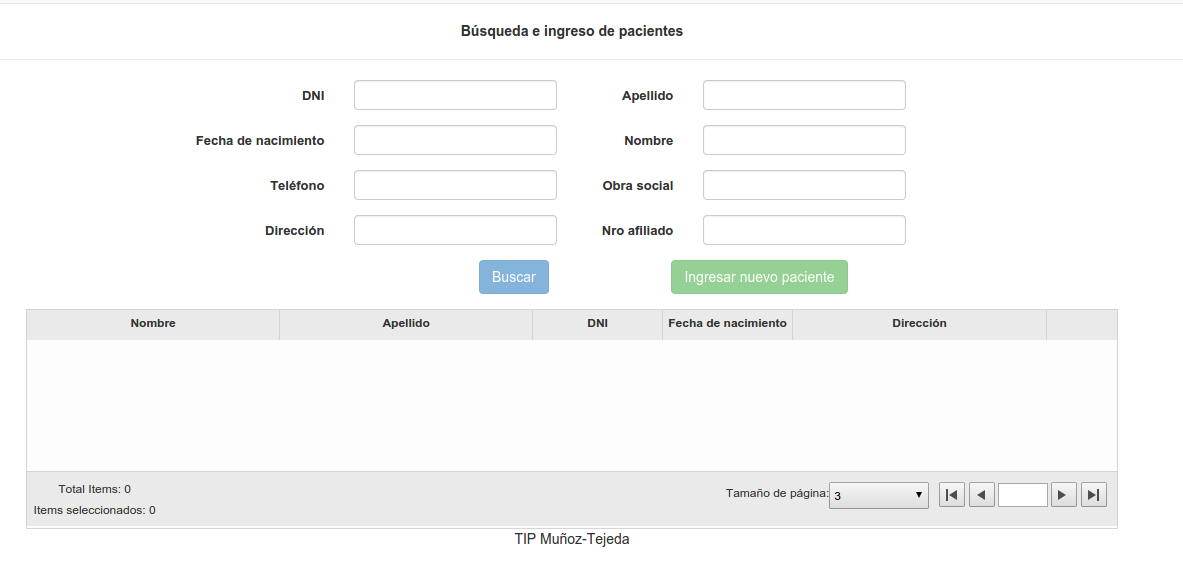
\includegraphics[width=0.99\textwidth]{inicio.png}}
\caption{Pantalla inicial} \label{fig:inicio}
\end{figure}
se pueden ver los campos identitificatorios de las personas. El botón ``Ingresar nuevo paciente'' aparecerá deshabilitado hasta completar los campos obligatorios: DNI, nombre, apellido y fecha de nacimiento (como puede verse en la figura \ref{fig:inicio_nuevo}).
\begin{figure}
\centerline{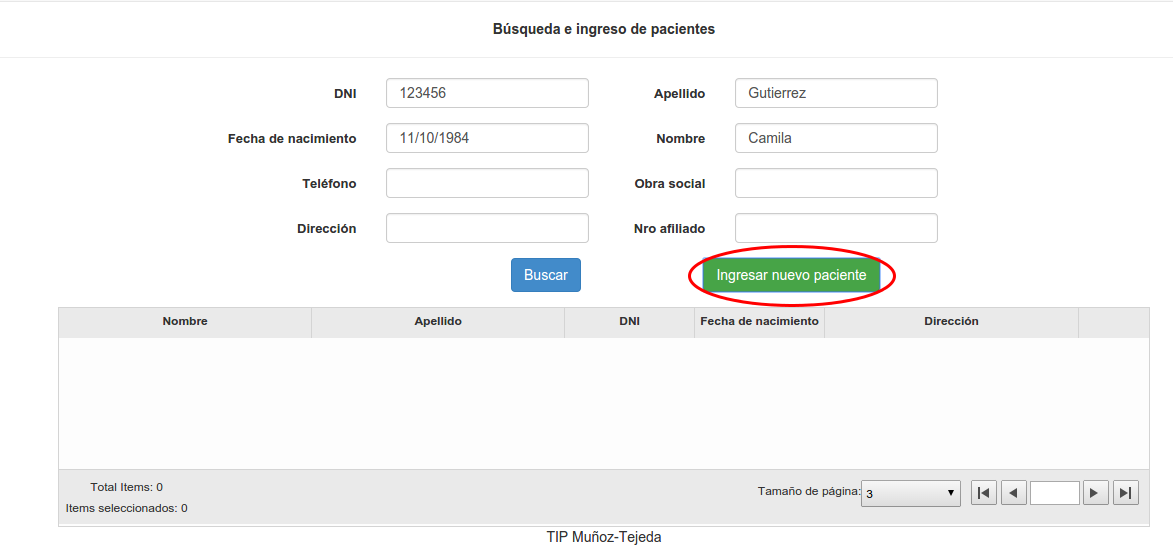
\includegraphics[width=0.99\textwidth]{inicio_nuevo.png}}
\caption{Botón habilitado para poder cargar nuevo paciente} \label{fig:inicio_nuevo}
\end{figure}
Al presionar dicho botón, el sistema guardará los datos de esa persona y redigirá la aplicación a la ventana de Triage para comenzar con la carga de síntomas.

\mySubSection{Búsqueda e ingreso de un paciente cargado en sistema}
En el caso de que el paciente ya haya recibido atención en la guardia, es posible buscarlo en la aplicación. El botón ``buscar'' apacerá deshabilitado hasta que se complete alguno de los campos (figura \ref{fig:inicio_busqueda}).
\begin{figure}
\centerline{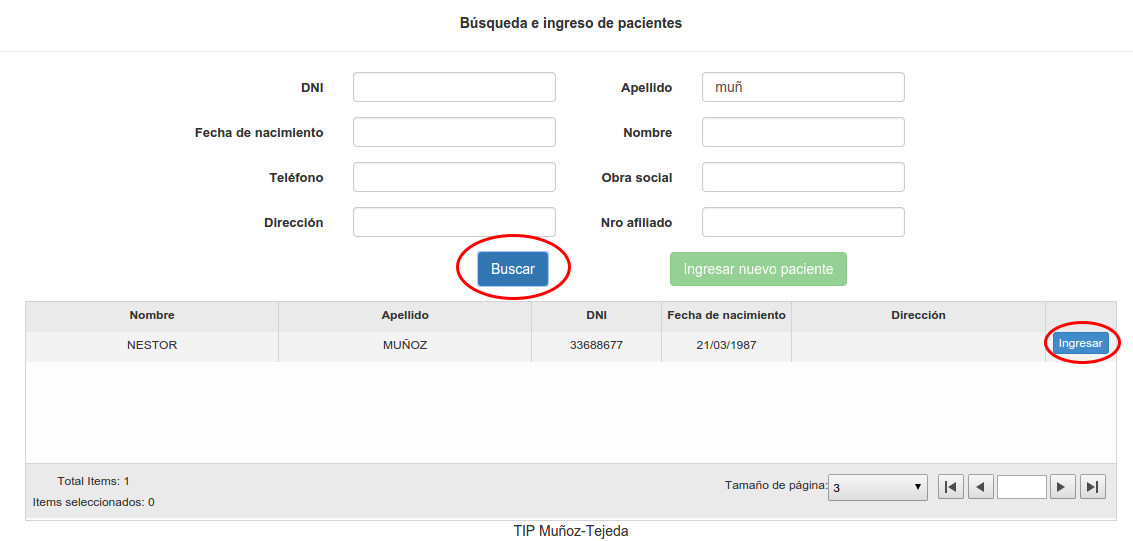
\includegraphics[width=0.99\textwidth]{inicio_busqueda.png}}
\caption{Botón habilitado para poder buscar un paciente y botón para ingresar al paciente a Triage} \label{fig:inicio_busqueda}
\end{figure}
Una vez presionado el botón para buscar, el sistema muestra en el listado inferior la lista de personas que coinciden con los criterios de búsqueda ingresados (ver sección \ref{cap:filtrado_listado}). En el caso de ver a la persona que se está buscando, en la lista aparece el botón ``Ingresar''. Al presionarlo, el sistema redirige la aplicación a la ventana de Triage para comenzar con la carga de síntomas.

\mySubSection{Filtrado de un listado}\label{cap:filtrado_listado}
Todos los listados de la aplicación pueden ser filtrados para facilitar la búsqueda de algún registro. El modo de filtrado es muy sencillo. Los pasos a seguir son los siguientes:
\begin{enumerate}
\item ingresamos algun texto en el/los campo/s de búsqueda (no hace falta que ingresemos la palabra entera de lo que buscamos, es suficiente si solo ingresamos las primeras letras)
\item presionamos el boton ``Buscar''
\end{enumerate}

